\documentclass[12pt,ngerman]{scrartcl}
\usepackage{tikz}
\usetikzlibrary{positioning}

\begin{document}

\begin{center}
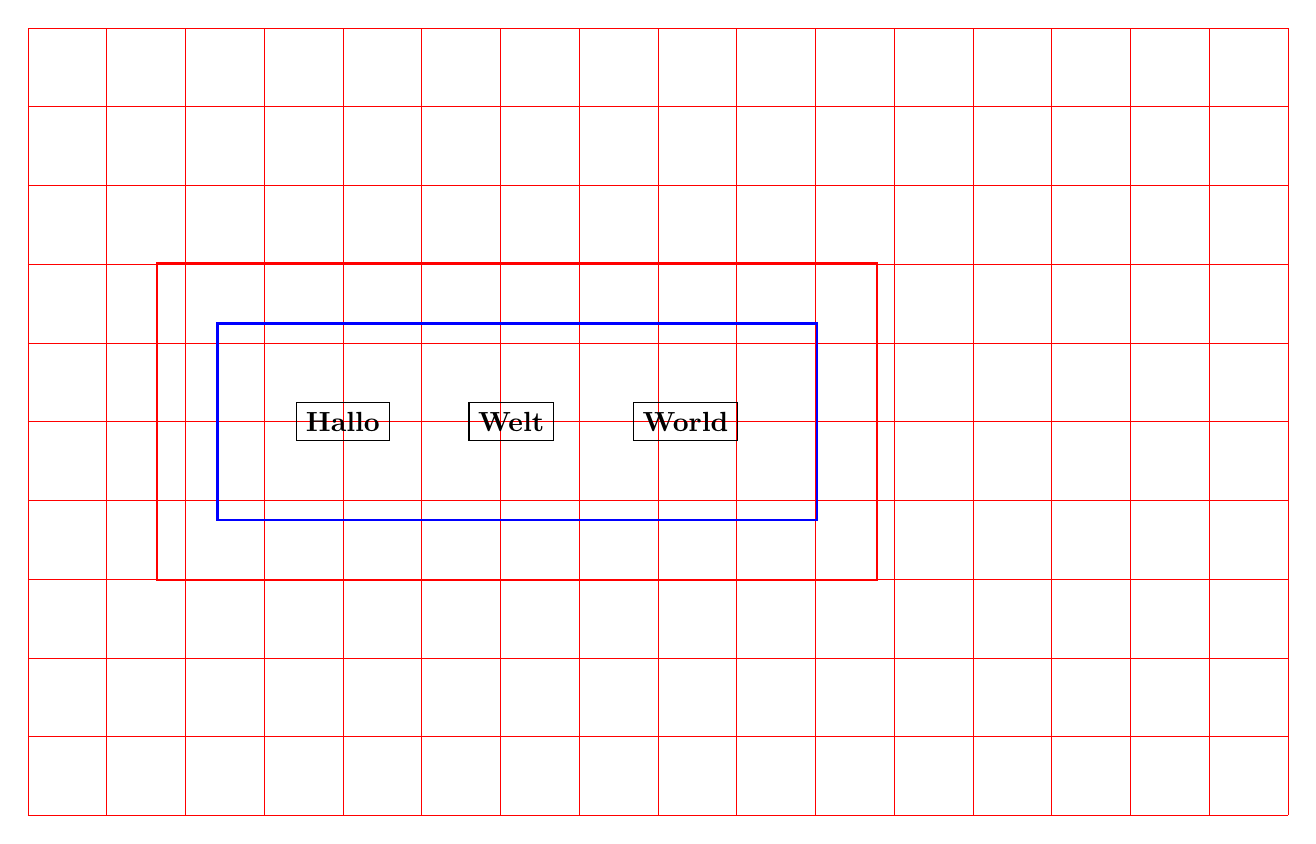
\begin{tikzpicture}
\draw[help lines,red] (0,0) grid (16,10);

\node[rectangle,draw,black](a) at (4,5){\bfseries Hallo}; 
\node [right =1cm of a,rectangle,draw,black] (b) {\bfseries Welt};
\node [right =1cm of b,rectangle,draw,black] (c) {\bfseries World};

% linke obere ecke
\coordinate [above left = of a.north west](loe);
% rechte untere ecke
\coordinate [below right= of c.south east](rue);

\draw [draw=blue,thick] (loe) rectangle (rue);

% linke obere ecke 25mm
\coordinate [above left = 25mm of a.north west](loe2);
% rechte untere ecke 25mm
\coordinate [below right= 25mm of c.south east](rue2);

\draw [draw=red,thick] (loe2) rectangle (rue2);





\end{tikzpicture}
\end{center}

\end{document}
